\section{Bartosz Pieczek}

\subsection{Albert Einstein i $E = mc^2$}

\hspace{\parindent}Albert Einstein jest najbardziej znany ze swojej teorii względności, zawartej w równaniu \( E = mc^2 \), które zrewolucjonizowało fizykę.\par\textbf{Albert Einstein} wprowadził nową perspektywę na \textbf{masę} i \textbf{energię}, pokazując, że są one \textit{równoważne}. Jego równanie stało się \textbf{fundamentem} współczesnej fizyki i wpłynęło na rozwój technologii, takich jak \textit{energia jądrowa}.


\subsection{Wyrażenie matematyczne}
Energia (\( E \)) obiektu jest związana z jego masą (\( m \)) oraz prędkością światła (\( c \)) według wzoru:
\[
E = mc^2
\]

\subsection{Obraz}
Na rysunku \ref{fig:einstein} przedstawiono znane zdjęcie Alberta Einsteina.

\begin{figure}[ht]
    \centering
    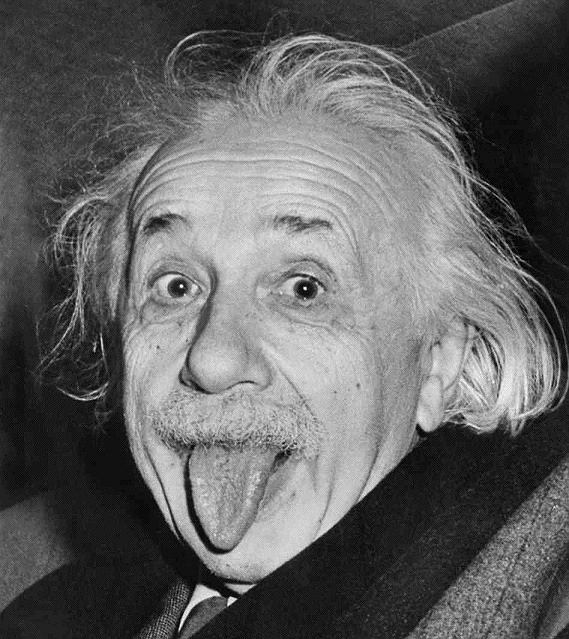
\includegraphics[width=0.5\textwidth]{pictures/einstein.jpg}
    \caption{Albert Einstein}
    \label{fig:einstein}
\end{figure}

\subsection{Lista numerowana:}
Przykład listy numerowanej:
\begin{enumerate}
    \item Albert Einstein urodził się w 1879 roku.
    \item Opracował teorię względności.
\end{enumerate}

\subsection{Tabela}
Tabela \ref{tab:mass-energy} przedstawia wartości związane z równaniem masy i energii.

\begin{table}[ht]
    \centering
    \begin{tabular}{|c|c|}
    \hline
    Masa (kg) & Energia (J) \\ \hline
    $1$        & $8.99 \times 10^{16}$ \\ \hline
    $10$       & $8.99 \times 10^{17}$ \\ \hline
    \end{tabular}
    \caption{Tabela masy i energii}
    \label{tab:mass-energy}
\end{table}


\subsection{Lista nienumerowana:}
I lista nienumerowana z pauzami:
\begin{itemize}
    \renewcommand\labelitemi{--}
    \item Równanie \( E = mc^2 \) zmieniło nasze rozumienie energii.
    \item Zasada ta dotyczy każdej materii.
\end{itemize}